\section{Distancias y superficies básicas}
En 2-D, La distancia entre $P_1(x_1,y_i)$ \& $P_2(x_2,y_2)$, se encontraba la distancia entre dos puntos estaba dada por el teorema de pitágoras. Para encontrar la distancia entre $\displaystyle P_1$ y $\displaystyle P_2$, se utiliza la fórmula:
\[
  d = \sqrt{\p{x_2-x_1} ^2 + \p{y_2-y_1} ^2}
\]
{
    \begin{figure}[!htb]
        \centering
        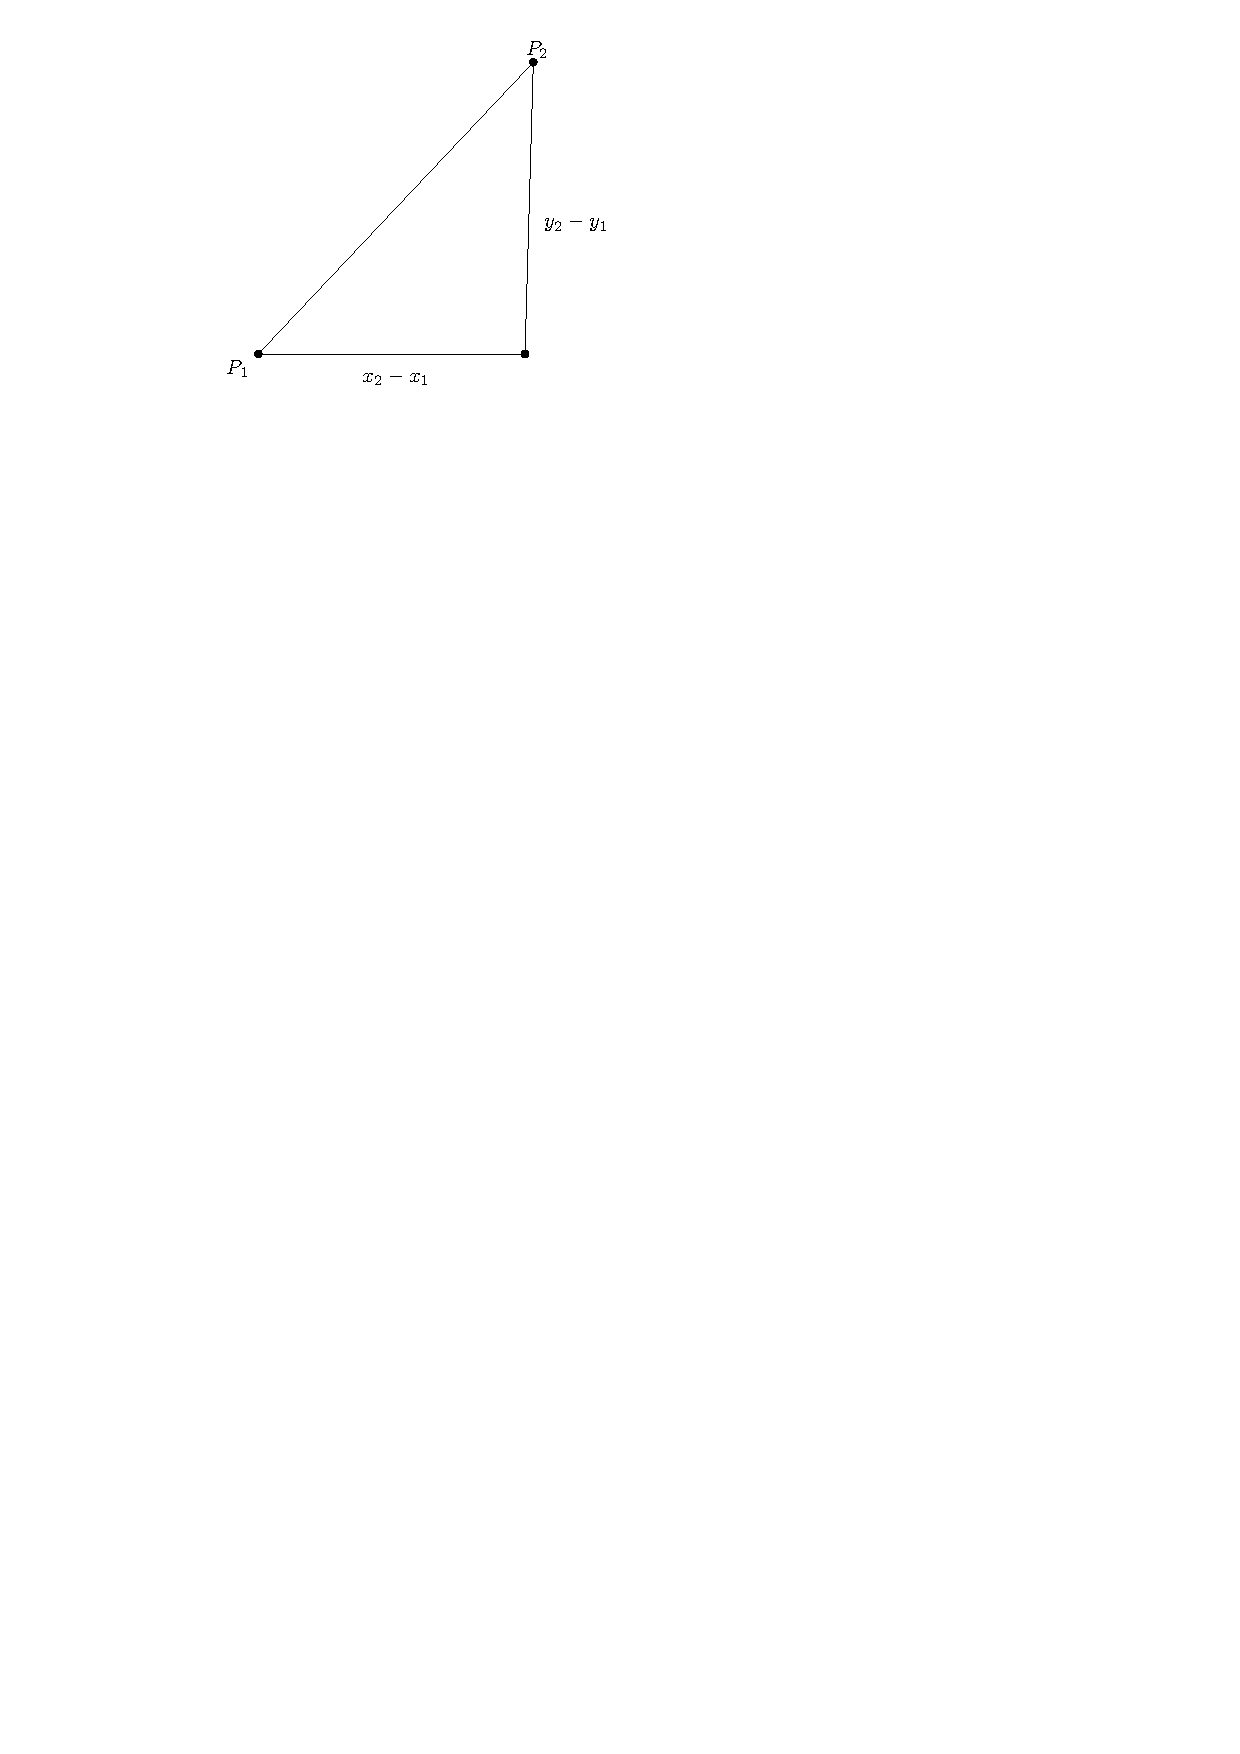
\includegraphics[scale=0.75]{Clases/figs/2020-01-23-01}  \qquad \qquad 
        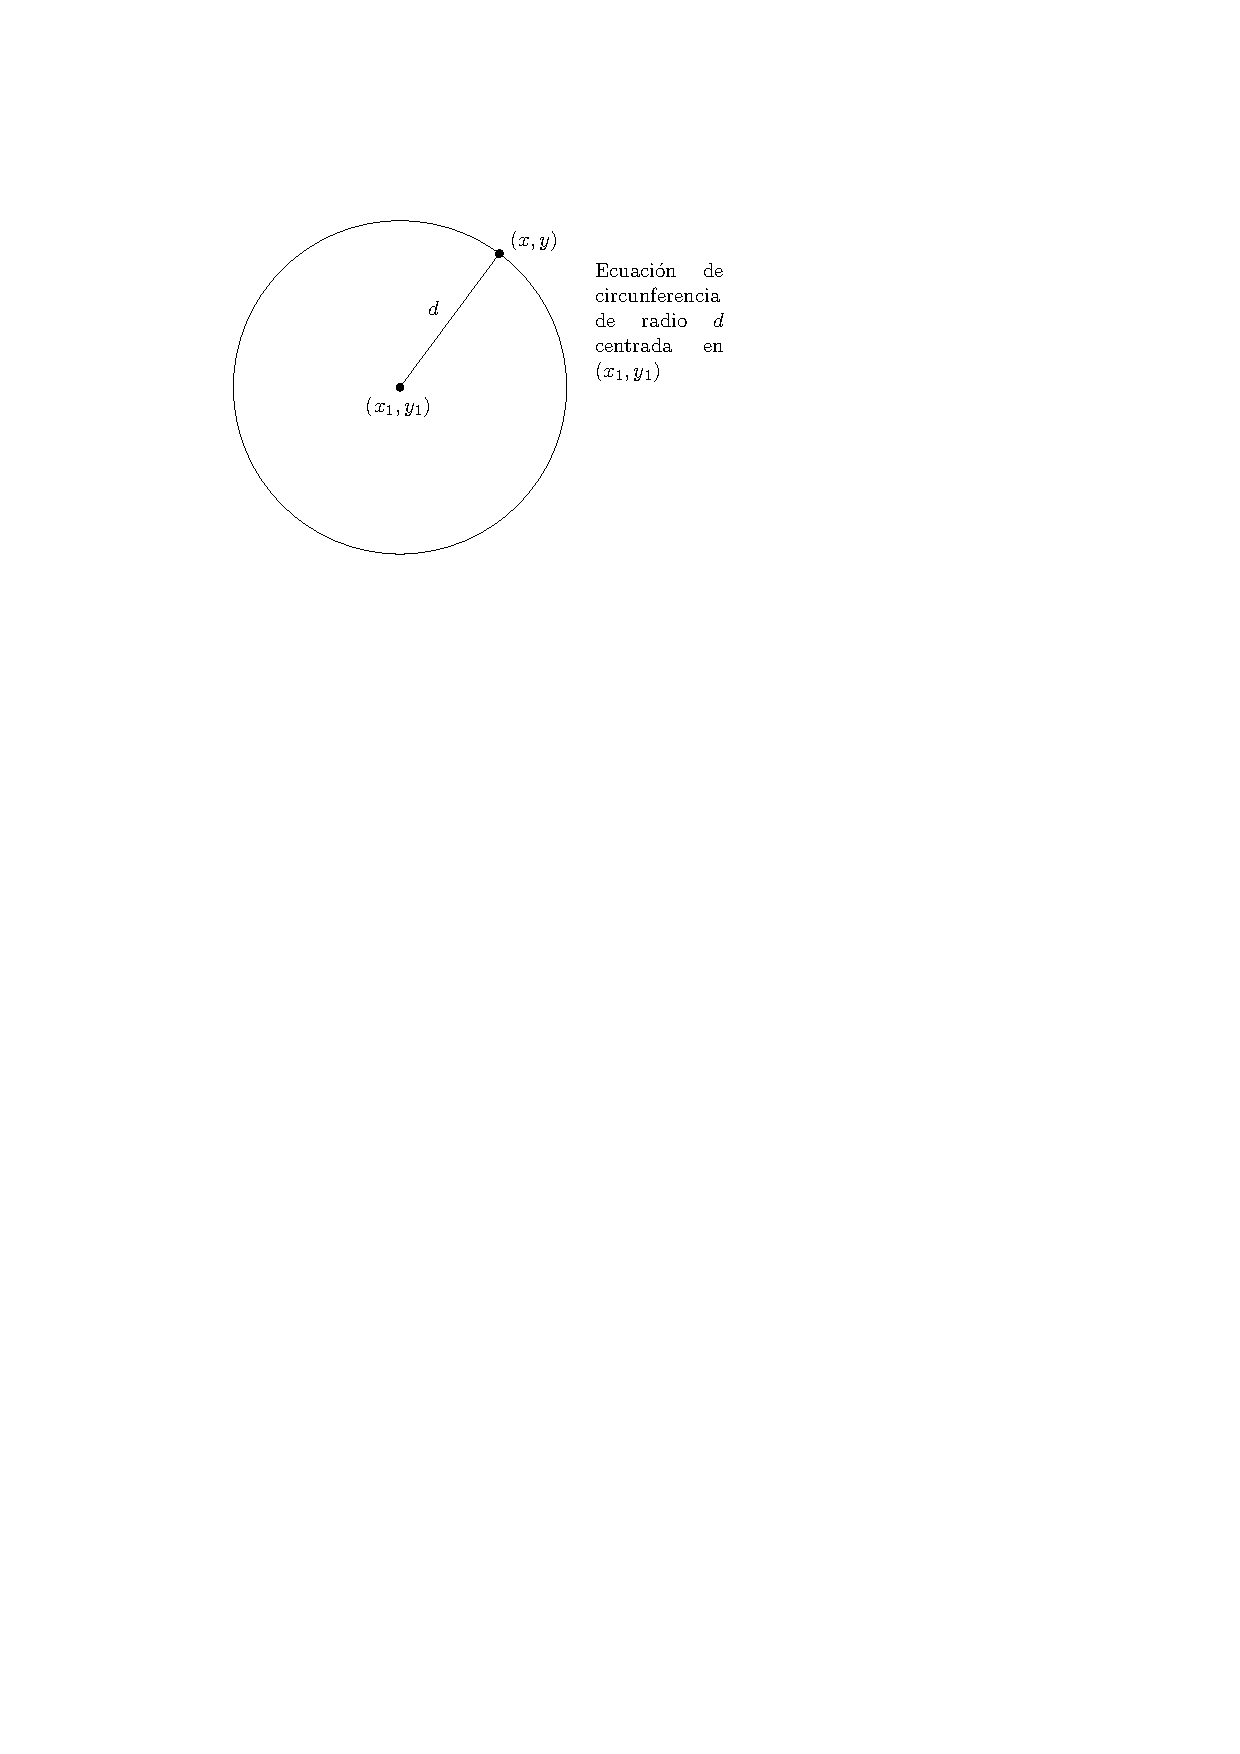
\includegraphics[scale=0.75]{Clases/figs/2020-01-23-02}
    \end{figure}
    
    En 3-D, para encontrar la diferencia entre $P_1(x_1,y_1,z_1)$ \& $P_2(x_2,y_2,z_2)$, calcule la diferencia entre $z_2$ y $z_1$.
    \[
        d = + \sqrt{(x_2-x_1)^2+(y_2-y_1)^2+(z_2-z_1)^2} 
    \]
}
{
    Tomar en cuenta que no puede ser negativa. \newline Para denotar la distancia entre $\displaystyle P_1,P_2$ se denota como: $\displaystyle d = \absval{P_2 P_1} $ 

    \begin{center}
        \begin{figure}[H]
            \centering
            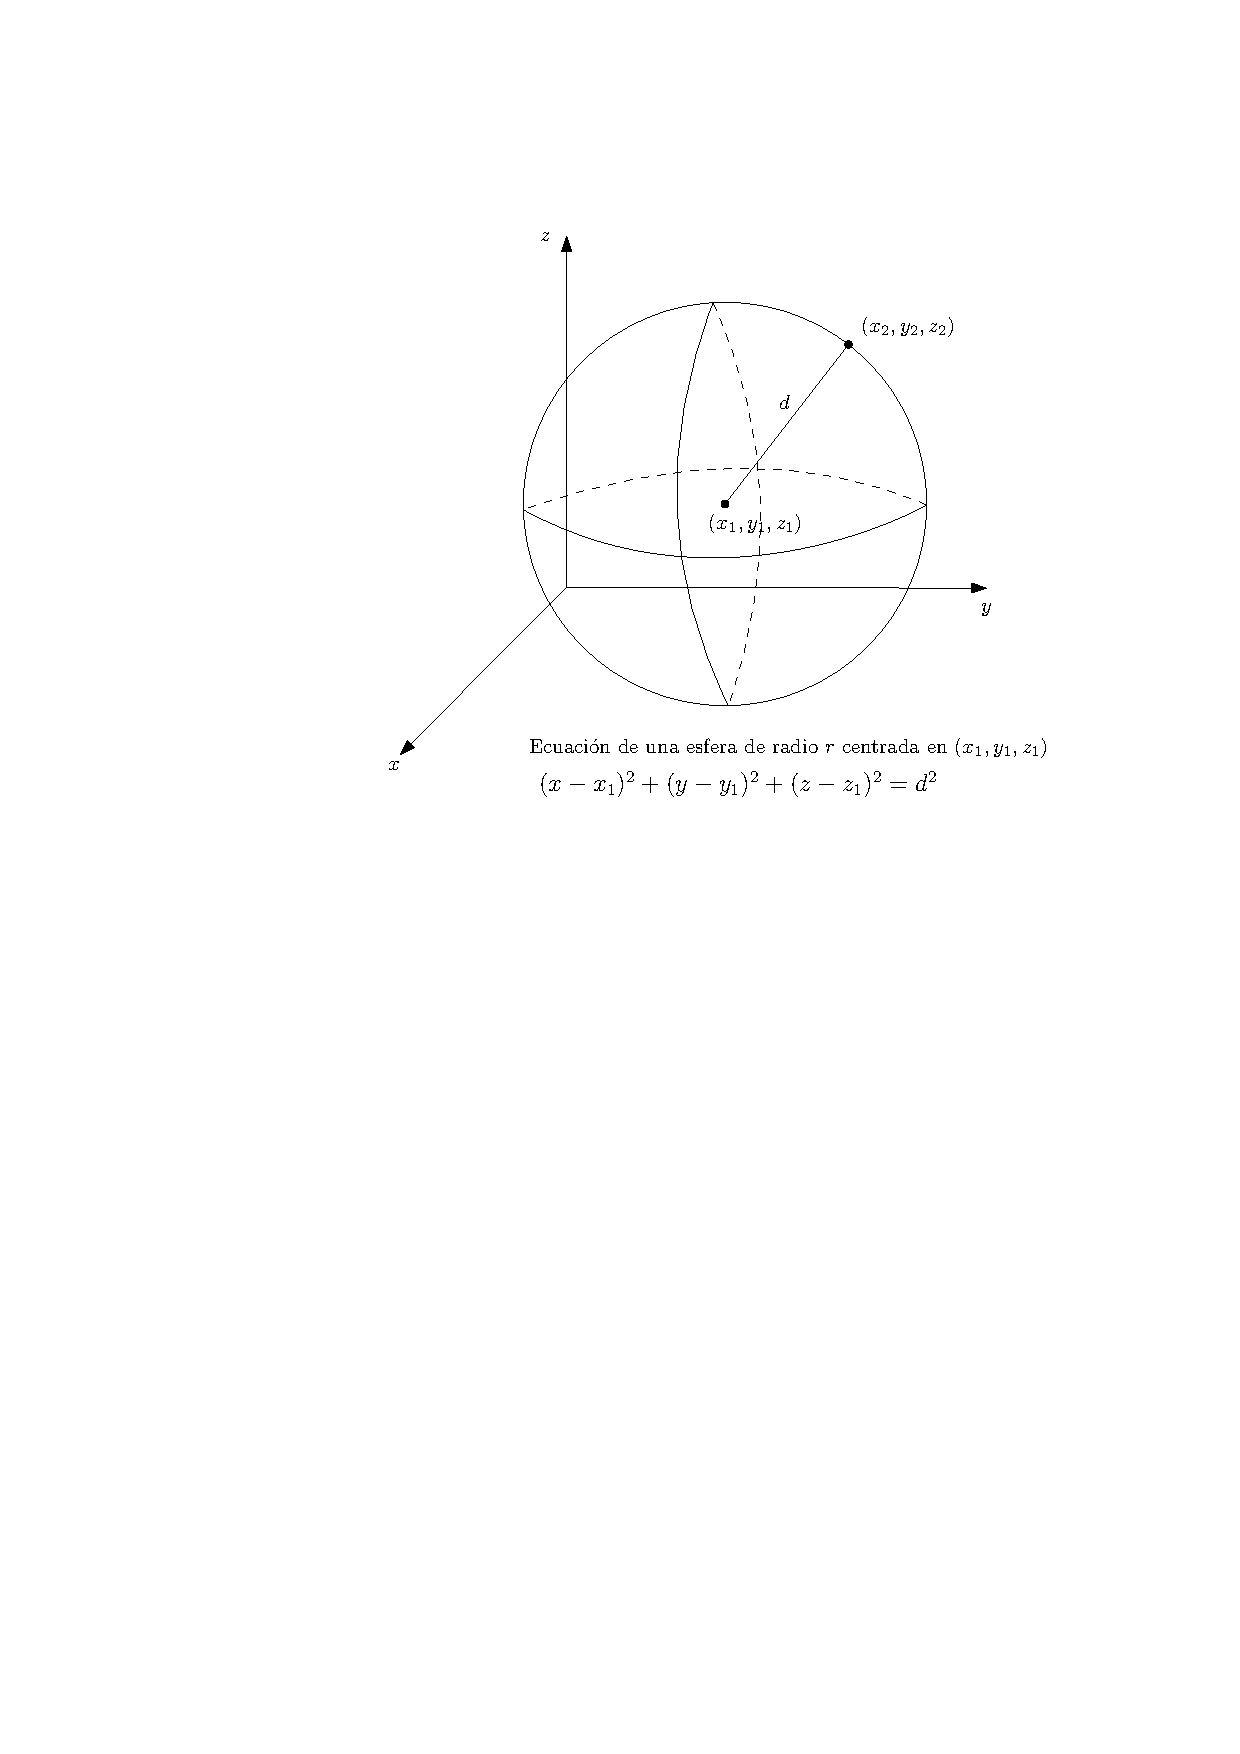
\includegraphics[scale=0.75]{Clases/figs/2020-01-23-03} 
            \caption{La esfera centrada en $(x_1,y_2,z_2)$} 
        \end{figure}
    \end{center}
}
%%%%%%%%%%%%%%%%%%%%%%%%%%%%%%%%%%%%%%%%%%%%%%%%%%%%%%%%%%%%%%%%%%%%%%%%%%%%%%%%%%%%%%%%%%%%%%%%
% \newpage 
\section{Ejercicios}
\begin{itemize}
    \item Encuentre el centro y radio de la esfera cuya ecuación es: 
        \[
            x^2+y^2+z^2+8x-6y+4z+4=0
        \]
        \begin{itemize}
            \item Tener en cuenta que es como que si estuviesen desarrollando la ecuación $x^2+y^2+z^2=r^2$ y agregando constantes.
            \item Hay que \textbf{completar al cuadrado}.
        \end{itemize}

        \begin{center}
            \begin{align*}
                x^2+y^2+z^2+8x-6y+4z+4&=0 \\ 
                x^2+8x+\square+y^2-6y+\square+z^2+4z+\square&=-4 \\ 
                \begin{matrix}
                    \text{  Para x:  }\, \left(\frac{8}{2}\right)^2 &= 16 \\ 
                    \text{  Para y:  }\, \left( \frac{6}{2}  \right)^2 &= 9 \\ 
                    \text{  Para z:  }\, \left(\frac{4}{2}\right)^2 &= 4 \\ 
                \end{matrix} \\ 
                x^2+8x+16+y^2-6y+9+z^2+4z+4&= -4 +16+9+4\\
                (x+4)^2+(y-3)^2+(z+2)^2&= \underbrace{25}_{r^2} \\ 
                \therefore \, \text{  La esfera se enfoca en centro:  }: (-4,3,-2) \\ 
                \therefore \text{  Radio:  } \, \sqrt[]{25}=5 \\ 
            \end{align*}
        \end{center}
        
        \begin{itemize}
            \item Tener en cuenta que $z=x^2+y^2$ no es una esfera, es una paraboloide.
        \end{itemize}
    
    \item Encontrar la distancia entre un punto y un plano coordenado, encuentre la distancia entre el punto $(1,3,5)$ y el plano $xz$.
        \begin{itemize}
            \item Vamos a estrellar ese punto contra el eje $xz$, la proyección del punto $P$ sobre el plano.
        \end{itemize}
        \begin{align*}
            \text{  Distancia entre   }\,\, P_1,P_2 \quad d=\sqrt[]{(1-0)^2+(3-0)^2+(5-5)^2} \\ 
            \text{  La proyección del punto (a,b,c) sobre el plano xz es el punto (a,0,c).  }\\ 
            \therefore \quad \text{  La distancia mínima entre p y el plano es:  } \\ 
            d=\left| 0+b^2+0 \right| = \left| b \right| \\ 
        \end{align*}
    
    
    \item ¿Cuál es la distancia entre el punto (1,3,5) y el plano xy?
        \begin{itemize}
            \item Asumo z=0
        \end{itemize}
        \begin{center}
           \begin{align*}
               d_{min}=&\sqrt[]{0+0+5^2}\\ 
               d_{min}=&5 \\ 
           \end{align*}
        \end{center}
    
    \item Ejercicio 6: Considere los puntos $A(3,0,-4),B(9,0,0)$ Y $C(0,1,\sqrt[]{15})$:    
        \begin{itemize}
            \item ¿Cuáles de los siguientes puntos está más cercano al origen?
            \item Hay que calcular la distancia de cada punto respecto del origen $(0,0,0)$.
            \item El origen se denota como $O(0,0,0)$
        \end{itemize}
        \begin{center}
           \begin{align*}
               d_{AO} =& \left| AO \right| \sqrt[]{9+0+16}=\sqrt[]{25}=5 \\ 
               d_{BO} =& \left| BO \right|= \sqrt[]{81+0+0} = \sqrt[]{81} = 9 \\ 
                d_{CO} 0 \left| CO \right| =& \sqrt[]{0+1+15} = \sqrt[]{16}=4 \\ 
           \end{align*}
        \end{center}
        \begin{itemize}
            \item El punto $C$ es el más cercano al origen.
        \end{itemize}
        \begin{itemize}
            \item ¿Cuáles de los puntos están sobre el plano $yz$? 
            \item Se asume x: 0
            \item $A$ y $B$ no están sobre el plano $yz$ $x\neq 0$.
            \item El punto $C$ $(0,1,\sqrt[]{15})$ si están sobre el plano $yz$.
            \item ¿Cuáles de los puntos está más cercano al plano $yz$? x=0:
                \begin{itemize}
                    \item Dado a que el punto C está en el plano yz su distancia es 0 entonces ese es el más cercano.
                \end{itemize}
        \end{itemize}
\end{itemize}





